%==============================================================

\chapter{Other Similarity metrics and Feature Extraction Performance}\label{simmet}

\section{Test Datasets}

Chapter \ref{datasets} introduced a range of MIR datasets but not all are fitting to the problems this thesis evaluates. To test the algorithms on the one hand a lot of data is needed, so the Free Music Archive with its over 100000 songs would be a solid option for performance tests. However on the other hand the genre distribution in the FMA dataset is quite one sided. Most of the songs are tagged as experimental, electronic and rock. Also this dataset may not be really representative for actual popular music, a lot of the songs are live recordings with poor audio quality, possibly influencing the results.
The 1517 artists dataset offers 19 different genres with songs relatively equally distributed. For an objective evaluation of the proposed algorithms e.g. by genre recall this dataset is ideal. For cover song detection, the covers80 dataset is included as well.
The last source used in this thesis is the private music collection. This collection is biased towards metal music but due to the match with personal taste, it offers a subjective evaluation of the results of the similarity analysis. 
In conclusion that sums up to about 117000 songs for future performance tests and about 12000 songs for a detailed evaluation of the algorithms in this thesis.\\

\begin{table}[h]
	\caption{used music datasets}
	\label{used_dsets}
	\begin{center}
		\begin{tabular}{|c||c|}
			\hline
			fma & 106.733 Songs\\
			\hline
			private & 8484 Songs\\
			\hline
			1517 artists & 3180 Songs\\
			\hline
			covers80 & 160 Songs (80 originals + 80 covers)\\
			\hline
		\end{tabular}
	\end{center}
\end{table}

As mentioned in \ref{datasets} all albums from the private music collections are cataloged as well and the associated document is in the appendices. For the first tests an even smaller sample dataset containing 10 songs out of 10 different genres was created from the private music collection and the list with the belonging songs is also in the appendices.

\section{Feature Extraction Performance}

After evaluating the different features in the last three chapters, this one discusses the feature extraction process in detail. The post processing of the features like the note estimation from the chroma features and the calculation of statistic features from the mfccs was already explained in the previous chapters and is left out here. The full code is in the appendices.

\subsection{Librosa}

For most of the plots in the introduction section \ref{audiofeat} the python toolkit librosa was used because of its ease of use and very good documentation. The code example shows the necessary methods to extract the most important features like mfcc, chromagram and beats/ onsets.
\begin{pythonCode}
path = ('music/guitar2.mp3')
x, fs = librosa.load(path)
mfcc = librosa.feature.mfcc(y=x, sr=fs, n_mfcc=12)
onset_env = librosa.onset.onset_strength(x, fs, aggregate=np.median)
tempo, beats = librosa.beat.beat_track(onset_envelope=onset_env,sr=fs)
hop_length = 512
times = librosa.frames_to_time(np.arange(len(onset_env)), sr=fs, hop_length=hop_length)
chroma = librosa.feature.chroma_stft(x, fs)
\end{pythonCode}	
But when extracting features from batches of audio data the librosa library turned out to be very slow. For a very small dataset of 100 songs, the extraction of just the mean, variance and covariance of the mfccs and the estimated notes from the chromagram took about 48 minutes. 
For larger datasets like the 1517 artists dataset the feature extraction process would have taken about 22 hours. 

\subsection{Essentia}

\cite{audiofeattoolb} compares different Audio feature extraction toolboxes and shows that essentia is a much faster alternative to librosa due to the underlying C++ Code and provides even more features, but it is a bit less well documented and requires more effort in implementation at the same time.\\ 
In the end the code to extract the necessary features had to be rewritten for the usage of essentia due to the slow performance of librosa. Essentia offers two different ways to handle audio files. The first one is to use the essentia standard library. It offers similar methods to librosa and uses an imperative programming style. The audio file has to be read, sliced and preprocessed by hand. 
The second way is to use essentia streaming. Basically a network of connected algorithms is created and they handle and schedule the "how and when" whenever a process is called.

\subsubsection{Essentia Standard}

In the final extractor code the mfcc calculation and beat histogram estimation is done with the essenia standard library, because it offers a fast and easy way to implement the basic feature extraction tasks. 
\begin{pythonCode}
audio = es.MonoLoader(filename=path, sampleRate=fs)()
hamming_window = es.Windowing(type='hamming')
spectrum = es.Spectrum()
mfcc = es.MFCC(numberCoefficients=13)
frame_sz = 2048
hop_sz = 1024
mfccs = numpy.array([mfcc(spectrum(hamming_window(frame)))[1] 
	for frame in es.FrameGenerator(audio, frameSize=frame_sz, hopSize=hop_sz)])
rhythm_extractor = es.RhythmExtractor2013(method="multifeature")
bpm, beats, beats_confidence, _, beats_intervals = rhythm_extractor(audio)
peak1_bpm, peak1_weight, peak1_spread, peak2_bpm, peak2_weight, peak2_spread, histogram =
	es.BpmHistogramDescriptors()(beats_intervals)
\end{pythonCode}

\subsubsection{Essentia Streaming}

The essentia streaming library is used to calculate the chroma features in the final code. It eases up the filtering with the high- and a lowpass filter. The audio signal is passed through various stages of processing and ultimately resulting in the chroma features of the high-pass filtered audio signal. 
\begin{pythonCode}
loader = ess.MonoLoader(filename=path, sampleRate=44100)
HP = ess.HighPass(cutoffFrequency=128)
LP = ess.LowPass(cutoffFrequency=4096)
framecutter = ess.FrameCutter(frameSize=frameSize, hopSize=hopSize, silentFrames='noise')
windowing = ess.Windowing(type='blackmanharris62')
spectrum = ess.Spectrum()
spectralpeaks = ess.SpectralPeaks(orderBy='magnitude', magnitudeThreshold=0.00001, 
	minFrequency=20, maxFrequency=3500, maxPeaks=60)
hpcp = ess.HPCP()
hpcp_key = ess.HPCP(size=36, referenceFrequency=440, bandPreset=False, minFrequency=20,
	maxFrequency=3500, weightType='cosine', nonLinear=False, windowSize=1.)
key = ess.Key(profileType='edma', numHarmonics=4, pcpSize=36, slope=0.6, 
	usePolyphony=True, useThreeChords=True)
pool = essentia.Pool()
loader.audio >> HP.signal
HP.signal >> LP.signal
LP.signal >> framecutter.signal    
framecutter.frame >> windowing.frame >> spectrum.frame
spectrum.spectrum >> spectralpeaks.spectrum
spectralpeaks.magnitudes >> hpcp.magnitudes
spectralpeaks.frequencies >> hpcp.frequencies
spectralpeaks.magnitudes >> hpcp_key.magnitudes
spectralpeaks.frequencies >> hpcp_key.frequencies
hpcp_key.hpcp >> key.pcp
hpcp.hpcp >> (pool, 'tonal.hpcp')
essentia.run(loader)
chroma = pool['tonal.hpcp'].T
\end{pythonCode}	

\subsubsection{Essentia performance}

The calculation with the essentia library for 100 songs took less than half of the time librosa needed. This is a significant improvement, however the essentia library uses only one CPU core so that performance was further improved by using the parallel python library as presented in the next code snippet.

\subsection{Essentia parallel}

Multiple CPU cores get a part of the filelist of all songs and can compute the features fully parallel. 
\begin{pythonCode}
job_server = pp.Server()
job_server.set_ncpus(ncpus)
jobs = [ ]
for index in xrange(startjob, parts):
	starti = start+index*step
	endi = min(start+(index+1)*step, end)
	jobs.append(job_server.submit(parallel_python_process, (index, filelist[starti:endi],1,1,1,1,1)))
	gc.collect()
times = sum([job() for job in jobs])
job_server.print_stats()
\end{pythonCode}
The computation time takes about 15.4 seconds for per song and processor core. 
Using 4 CPU cores for 100 songs, the overall processing time could be reduced to about 385 seconds.

\begin{equation} \label{eq:parallelp}
time = \frac{\#songs}{\#CPUs} \cdot 15.4s
\end{equation}
Parallel python also opens up the possibility to use a cluster instead of a single node PC. 

\subsection{rp\_extractor}

For the extraction of the rhythm patterns and rhythm histrogram features as described in chapter \ref{rhythmsimc} the rp\_extractor tool provided by the TU Wien was used. Although running in parallel on all CPU cores on a single node, the extraction of the features from 100 songs takes about 442 seconds.

\subsection{performance}
\begin{figure}[htbp]
	\centering
	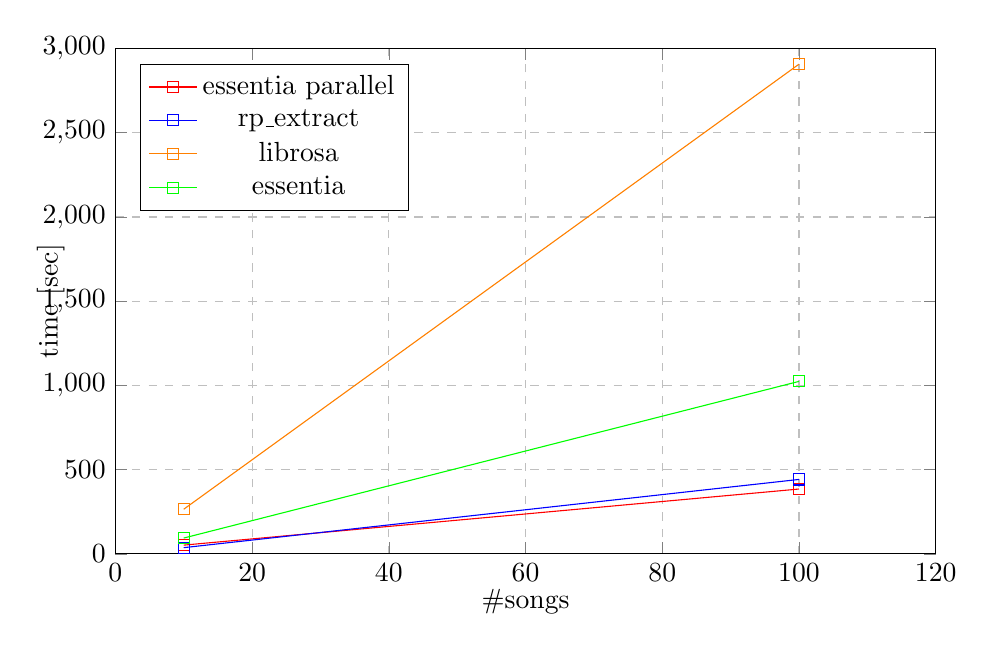
\begin{tikzpicture}
	\centering
	\begin{axis}[
	    %title={Performance of various toolkits},
		x label style={at={(axis description cs:0.5,-0.05)},anchor=north},
		y label style={at={(axis description cs:-0.05,.5)},rotate=0,anchor=south},
	    xlabel={\#songs},
	    ylabel={time [sec]},
	    xmin=0, xmax=120,
	    ymin=0, ymax=3000,
	    xtick={0,20,40,60,80,100,120},
	    ytick={0,500,1000,1500,2000,2500,3000},
	    legend pos=north west,
	    ymajorgrids=true,
	    grid style=dashed,
	    height=8cm,
	    width=12cm,
	    grid=major,
	]
	\addplot[
		color=red,
		mark=square,
		]
		coordinates {
		(10,52)(100,385)
		};
		\addlegendentry{essentia parallel}
	\addplot[
	    color=blue,
	    mark=square,
	    ]
	    coordinates {
	    (10,37)(100,442)
	    };
	    \addlegendentry{rp\_extract}
	\addplot[
	    color=orange,
	    mark=square,
	    ]
	    coordinates {
	    (10,265)(100,2907)
	    };
	    \addlegendentry{librosa}
	  
	\addplot[
	    color=green,
	    mark=square,
	    ]
	    coordinates {
		(10,94)(100,1024)
	    };
	    \addlegendentry{essentia}
	    
	\end{axis}
	\end{tikzpicture}
	\caption{Performance of various toolkits}
	\label{perfex}
\end{figure}
In summary the estimated time based on the performance measurements can be calculated and is listed below, leading to the conclusion that the extraction of the features for the full dataset including the FMA dataset can only be done with the help of a computing cluster or the FMA has to be left out. For this thesis the extracted features from the private music collection, the covers80 and the 1517 artists dataset summing up to over 11500 songs is more than sufficient and the FMA dataset is left out. For future work and performance testing however the inclusion of larger datasets has to be considered. 
\ \\
\ \\
\textbf{Estimated feature extraction times}
\begin{itemize}
	\item 3h24 - 1517 artists - essentia parallel, single node, 4 CPU cores
	\item 3h54 - 1517 artists - rp\_extract
	\item 9h06 - private dataset - essentia parallel, single node, 4 CPU cores
	\item 10h24 - private dataset - rp\_extract
	\item (125h - full dataset - essentia parallel, single node, 4 CPU cores)
	\item (143h - full dataset - rp\_extract)
\end{itemize}
